\documentclass[conference]{IEEEtran}
\IEEEoverridecommandlockouts
% The preceding line is only needed to identify funding in the first footnote. If that is unneeded, please comment it out.
%Template version as of 6/27/2024

\usepackage{cite}
\usepackage{amsmath,amssymb,amsfonts}
\usepackage{algorithmic}
\usepackage{graphicx}
\usepackage{float}
\usepackage{textcomp}
\usepackage{xcolor}
\usepackage[utf8]{inputenc}
\usepackage[spanish,es-tabla]{babel}
\usepackage{listings} 

\def\BibTeX{{\rm B\kern-.05em{\sc i\kern-.025em b}\kern-.08em
    T\kern-.1667em\lower.7ex\hbox{E}\kern-.125emX}}

\begin{document}

\title{Aprendiendo a jugar a Otelo: Agente Inteligente con Búsqueda Adversaria y Deep Learning}

\author{\IEEEauthorblockN{1\textsuperscript{st} Javier Luque Ruiz}
\IEEEauthorblockA{\textit{Grado en Ingeniería Informática - Ingeniería del Software} \\
\textit{Universidad de Sevilla}\\
Sevilla, España \\
javluqrui@alum.us.es}
}

\maketitle

\begin{abstract}
En este trabajo se explorará el desarrollo de un agente inteligente para el clásico juego de tablero Otelo (Reversi). 
El objetivo principal es construir un jugador capaz de tomar decisiones estratégicas mediante la implementación del 
algoritmo clásico de Minimax con poda alfa-beta para explorar el espacio de decisiones. Adicionalmente, se integrará 
una red neuronal profunda entrenada mediante autojuego para proporcionar una heurística de evaluación de las posiciones 
intermedias, reemplazando las funciones de evaluación manuales clásicas.
\end{abstract}

\begin{IEEEkeywords}
Inteligencia Artificial, Otelo, Reversi, Minimax, Poda Alfa-Beta, Deep Learning, Python.
\end{IEEEkeywords}

\section{Introducción}
El desarrollo de agentes inteligentes capaces de tomar decisiones estratégicas en juegos de tablero ha sido uno 
de los grandes hitos de la Inteligencia Artificial. Inspirado en los éxitos recientes de sistemas basados en 
aprendizaje profundo, este trabajo explora la combinación de algoritmos de búsqueda clásica con técnicas modernas de redes neuronales.

El objetivo principal de este proyecto es construir un agente inteligente para el clásico juego de Otelo (también conocido como Reversi). 
Específicamente, se aborda la variante del proyecto correspondiente a la convocatoria de julio, la cual requiere la implementación del 
algoritmo Minimax con poda alfa-beta para explorar el espacio de decisiones. La aportación central del sistema consiste en sustituir las 
funciones heurísticas manuales por una red neuronal profunda, la cual aprenderá a evaluar las posiciones intermedias del tablero basándose 
en un conjunto de datos generado mediante partidas de autojuego.

\section{Preeliminares}
\subsection{El juego de Otelo}
Otelo es un juego de estrategia de suma cero con información perfecta para dos jugadores, el cual se disputa sobre un tablero de $8 \times 8$ casillas. 
La partida inicializa con una disposición central de cuatro fichas cruzadas (dos blancas y dos negras), cediendo el primer movimiento al jugador con las piezas negras.

\begin{figure}[H]
    \centering
    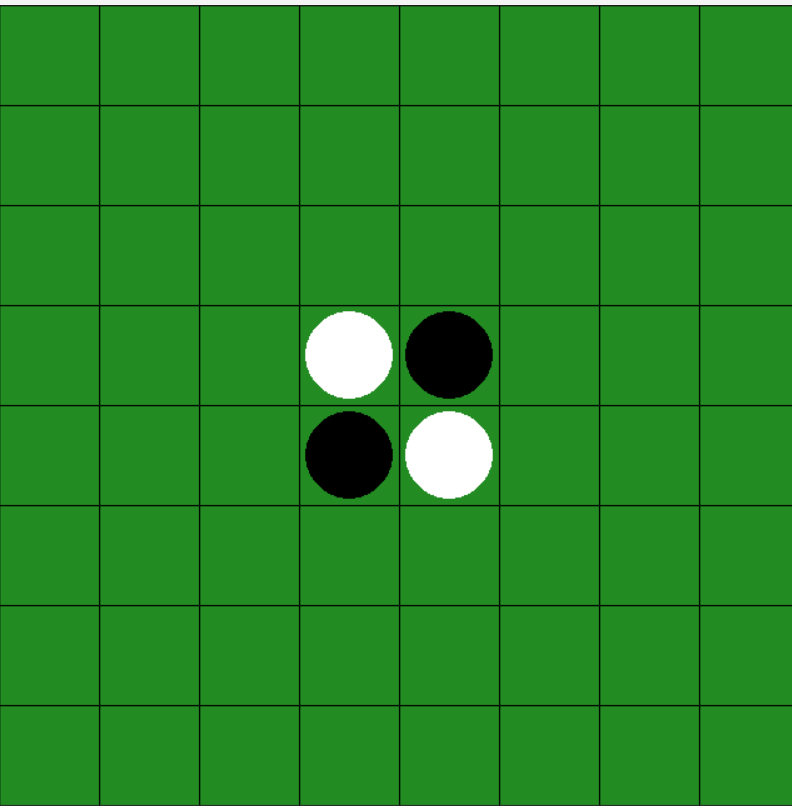
\includegraphics[width=0.25\textwidth]{images/otelo-posicioninicial.png}
    \caption{Tablero inicial de Otelo con la disposición central de fichas.}
    \label{fig:otelo_board}
\end{figure}

La mecánica central del juego es el \texttt{flanqueo}: un movimiento legal consiste en colocar una ficha en una casilla vacía de forma que, 
en línea recta (horizontal, vertical o diagonal), una o más piezas del oponente queden atrapadas entre la nueva ficha y otra pieza del 
jugador activo. Las fichas flanqueadas son capturadas y cambian de color. Si un jugador carece de movimientos legales, está obligado a 
pasar su turno. La partida concluye cuando el tablero se llena o ningún jugador puede realizar un movimiento válido, resultando ganador 
aquel con mayor número de fichas de su color.

\subsection{Búsqueda Adversaria y Poda Alfa-Beta}
El algoritmo Minimax es una técnica fundamental en la búsqueda adversaria que modela la toma de decisiones asumiendo que ambos jugadores 
actuarán de forma óptima: el agente intentará maximizar su puntuación (MAX) mientras que el oponente intentará minimizarla (MIN). Debido a 
que explorar el árbol de estados completo para Otelo es computacionalmente inabarcable, se implementa una estrategia de profundidad 
limitada (\textit{cutting-off search}). Al alcanzar dicha profundidad, el algoritmo detiene la simulación y evalúa la calidad del tablero mediante una heurística.

Para optimizar aún más los tiempos de respuesta, se aplica la poda alfa-beta. Esta mejora algorítmica mantiene el control de los 
peores escenarios posibles (los valores $\alpha$ y $\beta$) y descarta matemáticamente aquellas ramas del árbol que no influirán en la 
decisión final, reduciendo el número de estados evaluados sin alterar la optimalidad del movimiento elegido.


\section{Implementación}

\subsection{Motor del Juego}
Para la representación del tablero de Otelo se ha seleccionado una matriz bidimensional de $8 \times 8$ elementos utilizando la librería \texttt{NumPy}.
Esta decisión de diseño responde a la necesidad de gestionar los estados de forma eficiente y preparar los datos para su posterior tratamiento en la fase de Deep Learning.

De acuerdo con las especificaciones del enunciado del proyecto, se ha optado por utilizar la siguiente convención numérica para representar los distintos estados de las casillas:
\begin{itemize}
    \item \textbf{0}: Casilla vacía.
    \item \textbf{1}: Casilla ocupada por una ficha blanca.
    \item \textbf{2}: Casilla ocupada por una ficha negra.
\end{itemize}

La lógica de juego se encuentra en la clase \texttt{Otelo}. La validación de los movimientos se realiza mediante la función \texttt{es\_movimiento\_valido}, 
cuyo funcionamiento se basa en escanear las ocho direcciones posibles desde la casilla seleccionada empleando tuplas de desplazamiento:
\[
D = \{(0,1), (1,1), (1,0), (1,-1)
\]
\[
(0,-1), (-1,-1), (-1,0), (-1,1)\}
\]

Un movimiento se considera legal si, al recorrer una dirección, se encuentra al menos una ficha del oponente seguida de una ficha propia, sin que haya casillas vacías intermedias ni se 
salga del tablero. El método \texttt{ejecutar\_movimiento} aprovecha esta lógica para almacenar las coordenadas de las piezas atrapadas y actualiza el tablero en consecuencia, revertiendo las fichas del oponente a las propias.

\subsection{Interfaz Gráfica y Máquina de Estados}
La interacción con el usuario y la visualización del estado del juego se gestionan en el archivo \texttt{main.py} mediante la API gráfica de \texttt{PyGame}. 
Para evitar el acoplamiento de código y controlar de forma robusta el flujo de la aplicación, se ha diseñado una Arquitectura basada en una Máquina de Estados 
Estricta. El bucle principal del juego (\textit{Game Loop}) evalúa de forma continua los eventos del sistema y renderiza la interfaz basándose en el estado activo:

\begin{itemize}
    \item \textbf{\texttt{MENU}}: Pantalla de inicio que presenta el título y el botón para iniciar una nueva partida.
    \item \textbf{\texttt{JUGANDO}}: Estado activo durante el juego, donde se procesan los movimientos de los jugadores y se actualiza la visualización del tablero. Cuenta con un panel 
    inferior que muestra información relevante, como el turno actual y el marcador de fichas.
    \item \textbf{\texttt{PASAR\_TURNO}}: Estado crítico de validación que se activa cuando un jugador no tiene movimientos válidos disponibles, pero la partida continúa. En este estado,
    se notifica al jugador que está obligado a pasar turno mediante una confirmación explícita.
    \item \textbf{\texttt{FIN}}: Estado final que congela el estado del tablero y muestra el resultado de la partida, indicando el ganador o si ha habido un empate, así como el recuento final de fichas. 
\end{itemize}

\subsection{Agente Inteligente: Minimax con Poda Alfa-Beta}
Para dotar a la máquina de capacidad de decisión, se ha implementado un agente basado en el algoritmo Minimax complementado con la optimizacion de poda alfa-beta. 
Dado que el espacio de búsqueda de Otelo es considerablemente grande, el algoritmo se ejecuta con una profundidad limitada. Al alcanzar dicha profundidad, se aplica una función heurística
de evaluación manual básica, consistente en la diferencia de fichas entre el jugador maximizador y el minimizador. 

Durante la implementación del agente, se identificaron y resolvieron dos desafíos arquitectónicos principales para asegurar la robustez del agente:
\begin{itemize}
    \item \textbf{Gestión de turnos nulos en simulación}: En partidas avanzadas, es posible alcanzar estados donde un jugador no tiene movimientos válidos. Se implementó la lógica
    recursiva necesaria para que el agente ceda el turno de forma virtual en su árbol de búsqueda, en lugar de evaluar érroneamente esa rama como una derrota inmediata. Esto evita colapsos lógicos y la devolución de jugadas nulas al motor gráfico.
    \item \textbf{Ruptura del determinismo}: Al depender de una heurística simple de conteo de fichas, el agente podía generar movimientos repetitivos en situaciones de empate heurístico. 
    Se introdujo un mecanismo de aleatorización en la selección de movimientos cuando múltiples opciones presentaban la misma evaluación. Esta imprevisibilidad es un requisito técnico fundamental para garantizar una generación de datos heterogénea y rica durante la fase de autojuego para el posterior entrenamiento de la red neuronal.
\end{itemize}

\subsection{Generación del Conjunto de Datos mediante Autojuego}
Para entrenar la red neuronal, es necesario disponer de un conjunto de datos etiquetado que relacione estados del tablero con la calidad de la posición para el jugador activo. 
Dado que no existen bases de datos públicas de partidas de Otelo, se ha desarrollado un módulo de autojuego que enfrenta al agente Minimax contra sí mismo.

Se diseñó un entorno de simulación aislado de la interfaz gráfica donde dos agentes Minimax compiten entre sí. Durante la ejecución de cada partida, se registran los estados del 
tablero antes de cada movimiento junto al jugador activo.

Una vez finalizada la partida, se determina el ganador y se recorre el historial de estados para etiquetar cada posición con el resultado final desde la perspectiva del jugador activo en ese momento:
\begin{itemize}
    \item \textbf{+1}: Si el jugador activo ganó la partida.
    \item \textbf{0}: Si la partida terminó en empate.
    \item \textbf{-1}: Si el jugador activo perdió la partida.
\end{itemize}

Aprovechando la aleatoriedad introducida previamente en el agente para romper el determinismo, se simularon 500 partidas completas de forma automatizada, generando una base de 
datos heterogénea de aproximadamente 30.000 tableros. Para optimizar el rendimiento de lectura durante la fase de entrenamiento, las estructuras de datos se transformaron 
en tensores y se exportaron en formato binario nativo (\texttt{.npy}) haciendo uso de la librería \texttt{NumPy}, separando las características 
de entrada (matrices de estado) de las etiquetas de salida.

\subsection{Arquitectura y Entrenamiento de la Red Neuronal}
Una vez generado el conjunto de datos, se procedió a diseñar, compilar y entrenar una red neuronal profunda para aprender a evaluar las posiciones del tablero. Para ello, se utilizó la
interfaz de \texttt{Keras} sobre el motor \texttt{TensorFlow}. Siguiendo un enfoque alineado con las prácticas de la asignatura, se implementó un modelo secuencial con la siguiente arquitectura:
\begin{itemize}
    \item \textbf{Capa de Entrada y Aplanado}: Recibe la matriz del tablero de $8 \times 8$ casillas, la cual es procesada mediante una capa de aplanado (\texttt{Flatten}) para 
    convertirla en un vector unidimensional de 64 elementos.
    \item \textbf{Capas Ocultas}: Dos capas densas (\texttt{Dense}) con 64 y 32 neuronas respectivamente, ambas con función de activación ReLU para introducir no linealidad
    y evitar la saturación de gradientes.
    \item \textbf{Capa de Salida}: Una única neurona con función de activación de tangente hiperbólica (\texttt{tanh}), que devuelve un valor continuo en el rango [-1, 1], 
    representando la evaluación de la posición desde la perspectiva del jugador activo.
\end{itemize}

Para el proceso de optimización, se seleccionó el algoritmo de Descenso Estocástico por el Gradiente (SGD) con un factor de aprendizaje fijo de 0.01. La función de pérdida elegida fue
el Error Cuadrático Medio (MSE), evaluada conjuntamente con la métrica del Error Absoluto Medio (MAE). El entrenamiento se llevó a cabo durante 50 épocas con un tamaño de lote de 256 ejemplos, 
aplicando una división de 80\% para entrenamiento y 20\% para validación. 

\subsection{Análisis de Resultados y Evaluación del Modelo}
Tras completar las 50 épocas de entrenamiento, se observa que tanto el error de entrenamiento como el de validación se estabilizan en torno a valores de $0.97$ y $0.99$ respectivamente,
con un Error Absoluto Medio (MAE) final de aproximadamente $0.98$. Para entender mejor estos resultados, hay que recordar que las etiquetas del conjunto de datos oscilan entre $-1$ y $1$. Que 
el error medio sea cercano a $0.98$ indica que la red neuronal tiende a predecir valores cercanos a cero. En la práctica, esto significa que el modelo no se arriesga y evalúa la mayoría 
de las posiciones como estados de empate

Este resultado es coherente si analizamos la arquitectura elegida:
\begin{itemize}
    \item \textbf{Pérdida de la forma del tablero}: Al aplanar la matriz de $8 \times 8$ en un vector de 64 elementos, se pierde la información espacial y las relaciones entre las fichas adyacentes. Esto limita la capacidad del modelo para aprender patrones estratégicos complejos.
    \item \textbf{Capacidad de la red}: Con solo dos capas ocultas y un número limitado de neuronas, la red puede carecer de la complejidad necesaria para capturar las sutilezas del juego de Otelo, especialmente en posiciones intermedias donde la estrategia es crucial.
\end{itemize}

A pesar de esta limitación, el modelo entrenado puede servir como una primera aproximación para evaluar posiciones de manera rápida: toda la estructura de datos se ha comunicado correctamente,
el modelo ha entrenado de forma estable y el archivo resultante se ha integrado en tiempo real dentro del algoritmo Minimax.

\section{Pruebas y experimentación}
\section{Conclusiones}
\section{Bibliografía}

\begin{thebibliography}{00}
    \bibitem{russell} S. Russell and P. Norvig, \textit{Artificial Intelligence: A Modern Approach}, 4th ed., Pearson, 2020, ch. 5, ``Adversarial Search''.

\end{thebibliography}



\section*{References}

Please number citations consecutively within brackets \cite{b1}. The 
sentence punctuation follows the bracket \cite{b2}. Refer simply to the reference 
number, as in \cite{b3}---do not use ``Ref. \cite{b3}'' or ``reference \cite{b3}'' except at 
the beginning of a sentence: ``Reference \cite{b3} was the first $\ldots$''

Number footnotes separately in superscripts. Place the actual footnote at 
the bottom of the column in which it was cited. Do not put footnotes in the 
abstract or reference list. Use letters for table footnotes.

Unless there are six authors or more give all authors' names; do not use 
``et al.''. Papers that have not been published, even if they have been 
submitted for publication, should be cited as ``unpublished'' \cite{b4}. Papers 
that have been accepted for publication should be cited as ``in press'' \cite{b5}. 
Capitalize only the first word in a paper title, except for proper nouns and 
element symbols.

For papers published in translation journals, please give the English 
citation first, followed by the original foreign-language citation \cite{b6}.

\begin{thebibliography}{00}
\bibitem{otelo_rules} World Othello Federation, ``Othello Rules,'' [Online]. Disponible en: https://www.worldothello.org/about/about-othello/othello-rules\end{thebibliography}

\vspace{12pt}
\color{red}
IEEE conference templates contain guidance text for composing and formatting conference papers. Please ensure that all template text is removed from your conference paper prior to submission to the conference. Failure to remove the template text from your paper may result in your paper not being published.

\end{document}
